


%_______________
\newpage\subsection*{Exercises} % Considering categorical data

% 1

\eoce{\qt{Antibiotic use in children\label{antibiotic_use_children}} The bar plot 
and the pie chart below show the distribution of pre-existing medical 
conditions of children involved in a study on the optimal duration of 
antibiotic use in treatment of tracheitis, which is an upper respiratory 
infection.
\begin{center}
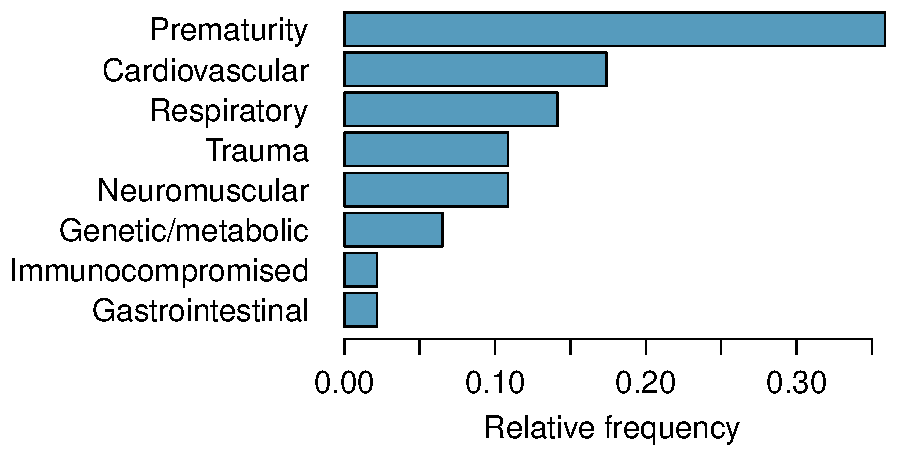
\includegraphics[width = 0.45\textwidth]{ch_summarizing_data/figures/eoce/antibiotic_use_children/antibiotic_use_children_bar}
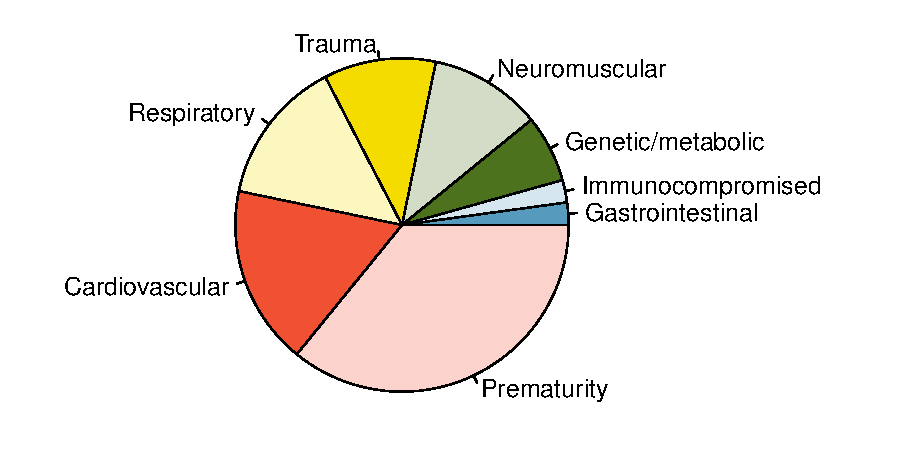
\includegraphics[width = 0.45\textwidth]{ch_summarizing_data/figures/eoce/antibiotic_use_children/antibiotic_use_children_pie}
\end{center}
\begin{parts}
\item What features are apparent in the bar plot but not in the pie chart?
\item What features are apparent in the pie chart but not in the bar plot?
\item Which graph would you prefer to use for displaying these categorical data?
\end{parts}
}{}

% 2

\eoce{\qt{Views on immigration\label{immigration}} 910 randomly sampled registered 
voters from Tampa, FL were asked if they thought workers who have illegally 
entered the US should be (i) allowed to keep their jobs and apply for 
US citizenship, (ii) allowed to keep their jobs as temporary guest workers 
but not allowed to apply for US citizenship, or (iii) lose their jobs and 
have to leave the country. The results of the survey by political ideology 
are shown below.\footfullcite{survey:immigFL:2012}
\begin{center}
\begin{tabular}{l l c c c c}
                        &                           & \multicolumn{3}{c}{\textit{Political ideology}} \\
\cline{3-5}
                        &                           & Conservative  & Moderate  & Liberal   & Total \\
\cline{2-6}
                        & (i) Apply for citizenship & 57            & 120       & 101       & 278 \\
                        & (ii) Guest worker         & 121           & 113       & 28        & 262 \\
\raisebox{1.5ex}[0pt]{\emph{Response}} & (iii) Leave the country    & 179       & 126       & 45        & 350 \\ 
                        & (iv) Not sure             & 15            & 4         & 1         & 20\\
\cline{2-6}
                        & Total                     & 372           & 363       & 175       & 910
\end{tabular}
\end{center}
\begin{parts}
\item What percent of these Tampa, FL voters identify themselves as conservatives?
\item What percent of these Tampa, FL voters are in favor of the citizenship option?
\item What percent of these Tampa, FL voters identify themselves as conservatives 
and are in favor of the citizenship option?
\item What percent of these Tampa, FL voters who identify themselves as 
conservatives are also in favor of the citizenship option? What percent of 
moderates share this view? What percent of liberals share this view?
\item Do political ideology and views on immigration appear to be independent? 
Explain your reasoning.
\end{parts}
}{}

% 3

\eoce{\qt{Views on the DREAM Act\label{dream_act_mosaic}} A random sample of registered 
voters from Tampa, FL were asked if they support the DREAM Act, a proposed law which would provide a path to citizenship for people brought illegally to the US as children.
The survey also collected information on the political ideology of the respondents. 
Based on the mosaic plot shown below, do views on the DREAM Act and  
political ideology appear to be independent? Explain your reasoning.
\footfullcite{survey:immigFL:2012}
\begin{center}
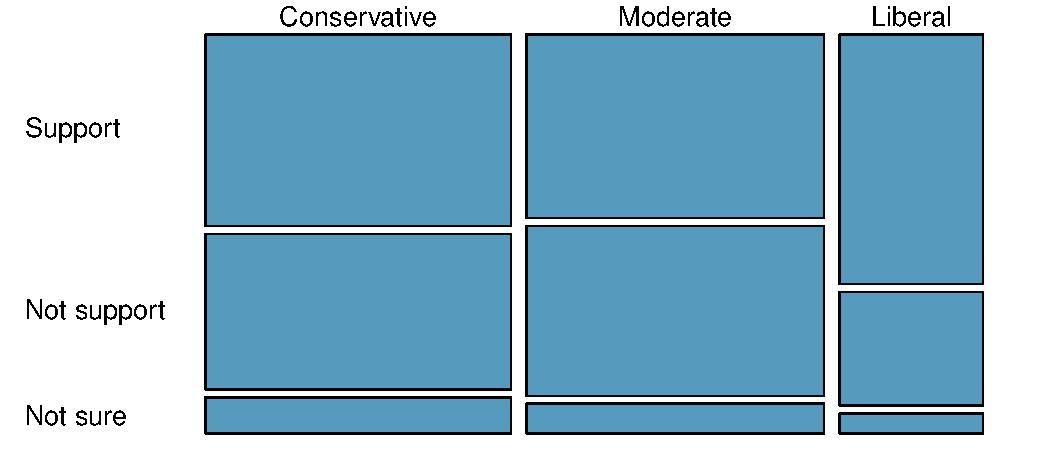
\includegraphics[width = 0.8\textwidth]{ch_summarizing_data/figures/eoce/dream_act_mosaic/dream_act_mosaic.pdf}
\end{center}
}{}

% 4

\eoce{\qt{Raise taxes\label{raise_taxes_mosaic}} A random sample of registered 
voters nationally were asked whether they think it's better to raise taxes 
on the rich or raise taxes on the poor. The survey also collected information 
on the political party affiliation of the respondents. Based on the mosaic 
plot shown below, do views on raising taxes and  
political affiliation appear to be independent? Explain your reasoning.
\footfullcite{survey:raiseTaxes:2015}
\begin{center}
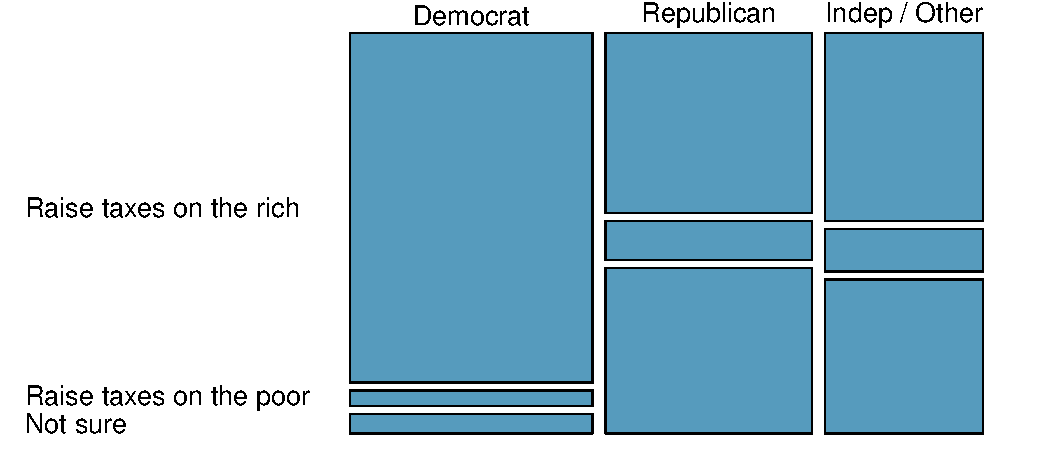
\includegraphics[width = 0.75\textwidth]{ch_summarizing_data/figures/eoce/raise_taxes_mosaic/raise_taxes_mosaic.pdf}
\end{center}
}{}
